\title{Aula 3 - Conceitos Básicos de Segurança da Informação}

\author{Prof. Gabriel Rodrigues Caldas de Aquino}

\institute
{
    Instituto de Computação \\
    Universidade Federal do Rio de Janeiro\\
    gabrielaquino@ic.ufrj.br % Your institution for the title page
}
\date{Compilado em: \\ \today} % Date, can be changed to a custom date

%----------------------------------------------------------------------------------------
%    PRESENTATION SLIDES
%----------------------------------------------------------------------------------------


\begin{frame}
    % Print the title page as the first slide
    \titlepage
\end{frame}




\begin{frame}{Disponibilidade}
\begin{itemize}
\item  Garante que os sistemas \textbf{funcionem} corretamente e que os serviços \textbf{não sejam negados} aos usuários autorizados.


    \item Não adianta ter dados íntegros e protegidos se o sistema está fora do ar.
\end{itemize}


   
\end{frame}



\begin{frame}{Disponibilidade em Segurança}
    \textbf{Disponibilidade} refere-se à capacidade de acessar a informação ou o recurso desejado quando necessário.

    \vspace{0.5cm}
    \begin{itemize}
        \item É essencial para a confiabilidade e o funcionamento do sistema.
        \item Um sistema indisponível é tão inútil quanto um sistema inexistente.
        \item Ataques como \textbf{DoS (Denial of Service)} exploram falhas de disponibilidade.
        \item Projetos de sistema geralmente assumem um \textit{modelo estatístico} de uso.
        \item Um atacante pode distorcer esse modelo (ex: tráfego de rede excessivo) para causar falhas.
    \end{itemize}

    \vspace{0.5cm}
    \textit{Se o sistema não foi projetado para o cenário de ataque, os mecanismos de proteção podem falhar.}
\end{frame}

\begin{frame}{Preocupação com Disponibilidade}
\centering

        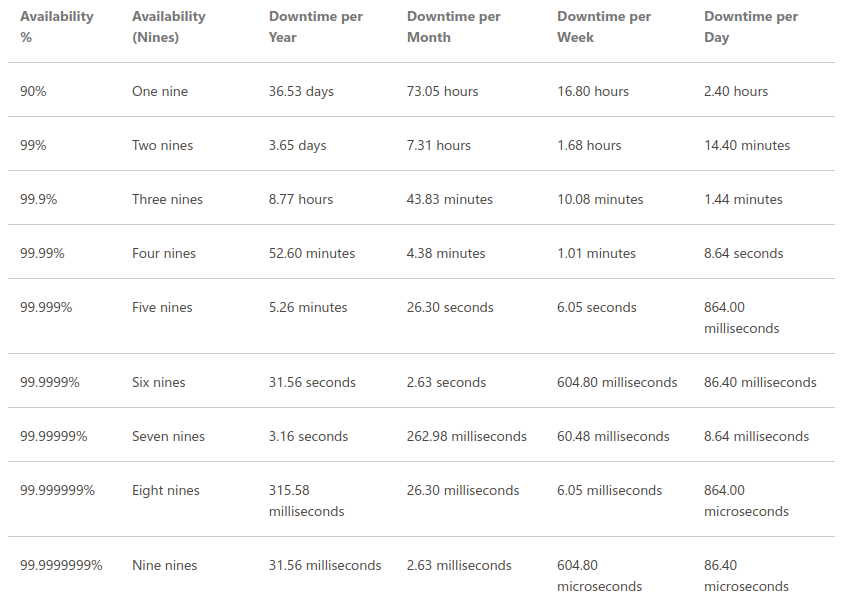
\includegraphics[width=0.7\linewidth]{Figuras/9s-disponibilidade.png}


\href{https://docs.oracle.com/en-us/iaas/Content/cloud-adoption-framework/high-availability.htm}{\textcolor{blue}{Link: Referência - Oracle}}

\end{frame}

\begin{frame}{De onde vêm os dados de disponibilidade?}
Seus cálculos de disponibilidade serão tão bons quanto os dados neles inseridos. Precisamos de dados  sobre interrupções e tempo de inatividade. 

Os dados de tempo de serviço e tempo de inatividade podem ser coletados de diversas fontes, incluindo:

\vspace{0.3cm}
\begin{itemize}
    \item Teste de ping
    \item Software de monitoramento
    \item Tickets de suporte técnico / call center
    \item Relatórios de TI quando ocorrem incidentes de interrupção
    \item Sistemas de Gestão de Informações e Eventos de Segurança (SIEMs)
    \item Análise de IA de arquivos de log e outras entradas e saídas do sistema
\end{itemize}


\end{frame}



\begin{frame}{Disponibilidade - Exemplo de Ataque DDoS}
  \begin{columns}[T]
    \begin{column}{0.48\textwidth}
      \begin{block}{\textbf{O Problema:}}
        \begin{itemize}
          \item \textbf{Cenário:} Sistema de matrículas online da universidade
          \item \textbf{Quando:} Primeiro dia do período de matrículas
          \item \textbf{Sintoma:} Sistema extremamente lento ou fora do ar
        \end{itemize}
      \end{block}
    \end{column}
    
    \begin{column}{0.48\textwidth}
      \begin{exampleblock}{\textbf{O Que Aconteceu?}}
        \begin{itemize}
          \item[•] Ataque DDoS (sobrecarga de acessos falsos)
          \item[•] +100.000 solicitações por segundo de bots
          \item[•] Servidores não conseguiram atender alunos reais
        \end{itemize}
      \end{exampleblock}
    \end{column}
  \end{columns}

  \begin{block}{\textbf{Soluções de prevenção e recuperação:}}
    \begin{columns}
      \begin{column}{0.5\textwidth}
      \begin{itemize}
          \item \textbf{Prevenção:}
        \begin{itemize}
          \item[•] Filtro contra tráfego malicioso
          \item[•] Limite de tentativas por IP
        \end{itemize}
      \end{itemize}
        
      \end{column}
      \begin{column}{0.5\textwidth}
      \begin{itemize}
          \item \textbf{Recuperação:}
        \begin{itemize}
          \item[•] Servidores reserva automáticos
          \item[•] Sistema prioritário para alunos cadastrados
        \end{itemize}
      \end{itemize}
        
      \end{column}
    \end{columns}
  \end{block}


\end{frame}

\begin{frame}{Dificuldade em Detectar Ataques de Negação de Serviço (DoS)}
    \begin{itemize}
        \item Ataques que visam tornar recursos indisponíveis são chamados de \textbf{ataques de negação de serviço (DoS)}.
        \item São \textbf{difíceis de detectar}, pois é necessário distinguir entre:
        \begin{itemize}
            \item Manipulação intencional de recursos ou do ambiente;
            \item Padrões de uso incomuns, mas legítimos.
        \end{itemize}
        \item Os modelos estatísticos usados para prever o uso normal:
        \begin{itemize}
            \item Consideram eventos atípicos como parte da distribuição estatística;
            \item Podem não identificar um ataque como anômalo.
        \end{itemize}
        \item Em alguns cenários, o ataque pode nem parecer atípico.
    \end{itemize}

    \begin{block}{Para detectar comportamentos estranhos na rede...}
        Precisamos ver os dados de funcionamento da rede
    \end{block}
\end{frame}

\begin{frame}{O que é um fluxo (flow) no NetFlow?}
Um \textit{flow} é definido como uma sequência unidirecional de pacotes com propriedades comuns que passam por um dispositivo de rede. Esses fluxos coletados são exportados para um dispositivo externo, o \textit{NetFlow collector}.

\vspace{0.3cm}
Um registro de fluxo inclui:
\begin{itemize}
    \item Endereços IP, Contagem de pacotes e bytes
    \item \textit{Timestamps}, Tipo de Serviço (ToS)
    \item Portas de aplicação, Interfaces de entrada e saída
\end{itemize}

\vspace{0.3cm}
Os dados exportados do NetFlow são usados para:
\begin{itemize}
    \item Faturamento de ISPs
    \item Monitoramento e planejamento de capacidade
    \item Monitoramento e perfil de aplicações e usuários
    \item Análise de segurança
    \item Mineração de dados para fins de marketing
\end{itemize}

\href{https://datatracker.ietf.org/doc/html/rfc3954}{\textcolor{blue}{Link: RFC 3954 -  NetFlow versão 9}}

\end{frame}


\begin{frame}{Dados da rede - O que é NetFlow?}
\begin{itemize}
    \item Protocolo de rede desenvolvido pela \textbf{Cisco Systems} para coletar metadados sobre o tráfego IP em roteadores, switches e hosts.
    \item Permite monitorar e obter conhecimento sobre o desempenho de aplicações e da rede.
    \item Fornece informações sobre:
    \begin{itemize}
        \item Quantidade de tráfego;
        \item Origem e destino do tráfego;
        \item Caminhos utilizados.
    \end{itemize}
    \item Estatísticas de fluxo ajudam no monitoramento, identificação de problemas e planejamento de upgrades.
\end{itemize}

\begin{itemize}
    \item \href{https://www.ibm.com/br-pt/think/topics/netflow}{\textcolor{blue}{Link: O que é o Netflow}}
    \item \href{https://www.ibm.com/docs/pt-br/npi/1.3.0?topic=devices-configuring-netflow-cisco-routers}{\textcolor{blue}{Link: Configurando o Netflow em roteadores CISCO}}
    \item \href{https://manpages.ubuntu.com/manpages/noble/man8/softflowd.8.html}{\textcolor{blue}{Link: Softflowd no Ubuntu}}
\end{itemize}
\end{frame}

\begin{frame}{Dados da rede - Como funciona o NetFlow}
\textbf{Principais componentes:}
\begin{enumerate}
    \item \textbf{Exportador de NetFlow:}
    \begin{itemize}
        \item Agrega pacotes em fluxos e exporta registros via UDP.
        \item Identifica fluxos com base em IP, portas, protocolo e tipo de serviço.
        \item Exporta fluxos inativos ou encerrados (ex: flags TCP FIN/RST).
    \end{itemize}
    
    \item \textbf{Dados da rede - Coletor NetFlow:}
    \begin{itemize}
        \item Recebe registros agregados de exportadores.
        \item Pré-processa e armazena os dados.
    \end{itemize}
    
    \item \textbf{Dados da rede - Analisador de NetFlow:}
    \begin{itemize}
        \item Processa e analisa os registros coletados.
        \item Gera relatórios e alertas sobre largura de banda, padrões de tráfego e uso de aplicações.
    \end{itemize}
\end{enumerate}
\end{frame}


\begin{frame}{Dados da rede - Solução NFSEN / NFDUMP}
    \textbf{NFDUMP}: Coleção de ferramentas para coleta e processamento de dados \textit{NetFlow} via linha de comando.  
    Faz parte do projeto \textbf{NfSen}. 

    \begin{itemize}
        \item  \href{https://github.com/phaag/nfdump}{\textcolor{blue}{Link: Github do projeto Nfdump}}
    \end{itemize}

   
    
    \vspace{0.3cm}
    \textbf{Principais ferramentas:}
    \begin{itemize}
        \item \textbf{nfcapd} — Daemon que captura fluxos de rede (\textit{NetFlow} v5, v7 e v9) e armazena em arquivos.
        \item \textbf{nfdump} — Lê e exibe dados \textit{NetFlow} dos arquivos, semelhante ao \textit{tcpdump}.
        \item \textbf{nfprofile} — Cria perfis de \textit{NetFlow} com base em filtros.
        \item \textbf{nfreplay} — Reenvia dados de fluxo para outro host.
        \item \textbf{nfclean.pl} — Limpa dados antigos de forma periódica.
        \item \textbf{ft2nfdump} — Converte dados de outras ferramentas de fluxo para o formato \textit{nfdump}.
    \end{itemize}
\end{frame}




\begin{frame}{Dados da rede - Arquitetura NFDUMP}
    \centering
    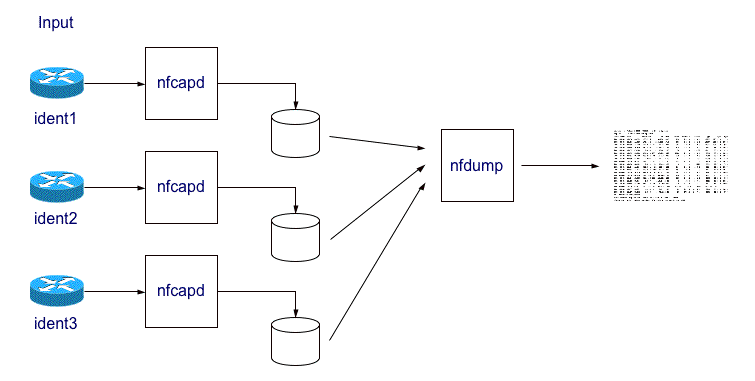
\includegraphics[width=0.85\linewidth]{Figuras/nfdump.png}
    \vspace{0.3cm}


\href{https://nfdump.sourceforge.net/}{\textcolor{blue}{Link: Ferramenta NFDUMP}}

\end{frame}

\begin{frame}{Dados da rede - Como o NFDUMP funciona}
    \centering
    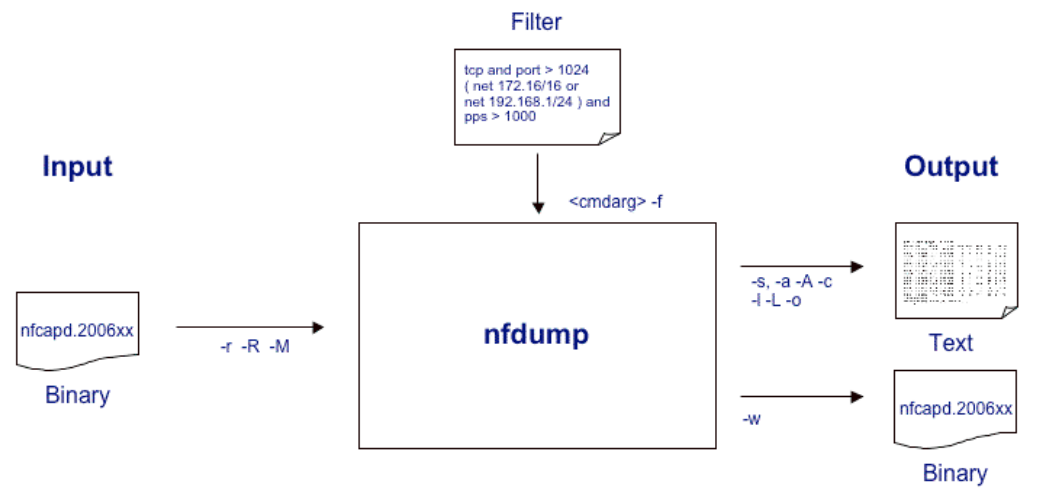
\includegraphics[width=0.85\linewidth]{Figuras/nfdump-filtros-processando.png}
    \vspace{0.3cm}


\href{https://www.first.org/resources/papers/conference2006/haag-peter-papers.pdf}{\textcolor{blue}{Link: User Documentation nfdump e NfSen}}

\end{frame}

\begin{frame}{Dados da rede - NfSen}
\textbf{Front-end gráfico baseado na Web} para as ferramentas de NetFlow do NFDUMP.

\vspace{0.5cm}
\textbf{Funcionalidades:}
\begin{itemize}
    \item Exibir e navegar facilmente pelos dados do NetFlow.
    \item Processar dados dentro de um período especificado.
    \item Criar histórico e perfis contínuos de tráfego.
    \item Definir alertas com base em várias condições.
    \item Desenvolver plugins personalizados para processar dados periodicamente.
\end{itemize}

\vspace{0.5cm}
\textit{Disponível no SourceForge, sob licença BSD.}

\begin{itemize}
    \item \href{https://sourceforge.net/projects/nfsen/}{\textcolor{blue}{Link: Sourceforge do NFSEN}}
\end{itemize}

\end{frame}

\begin{frame}{Dados da rede - Front-End Nfsen}
    \centering
    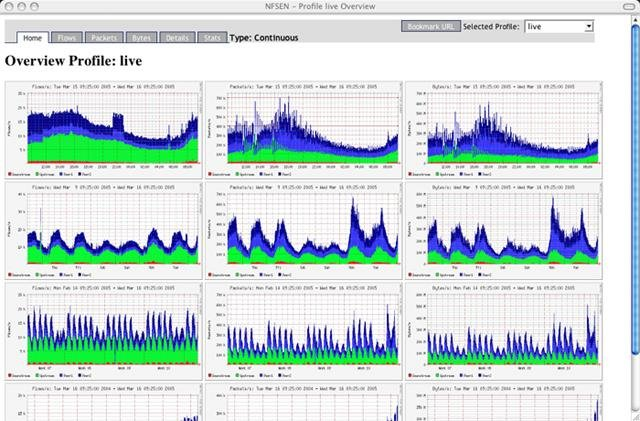
\includegraphics[width=0.75\linewidth]{Figuras/front-end-nfsen.png}
    \vspace{0.3cm}




\end{frame}


\begin{frame}{Dados da rede - Apresentação - Exemplo de uso NFSEN/NFDUMP}
    \centering
    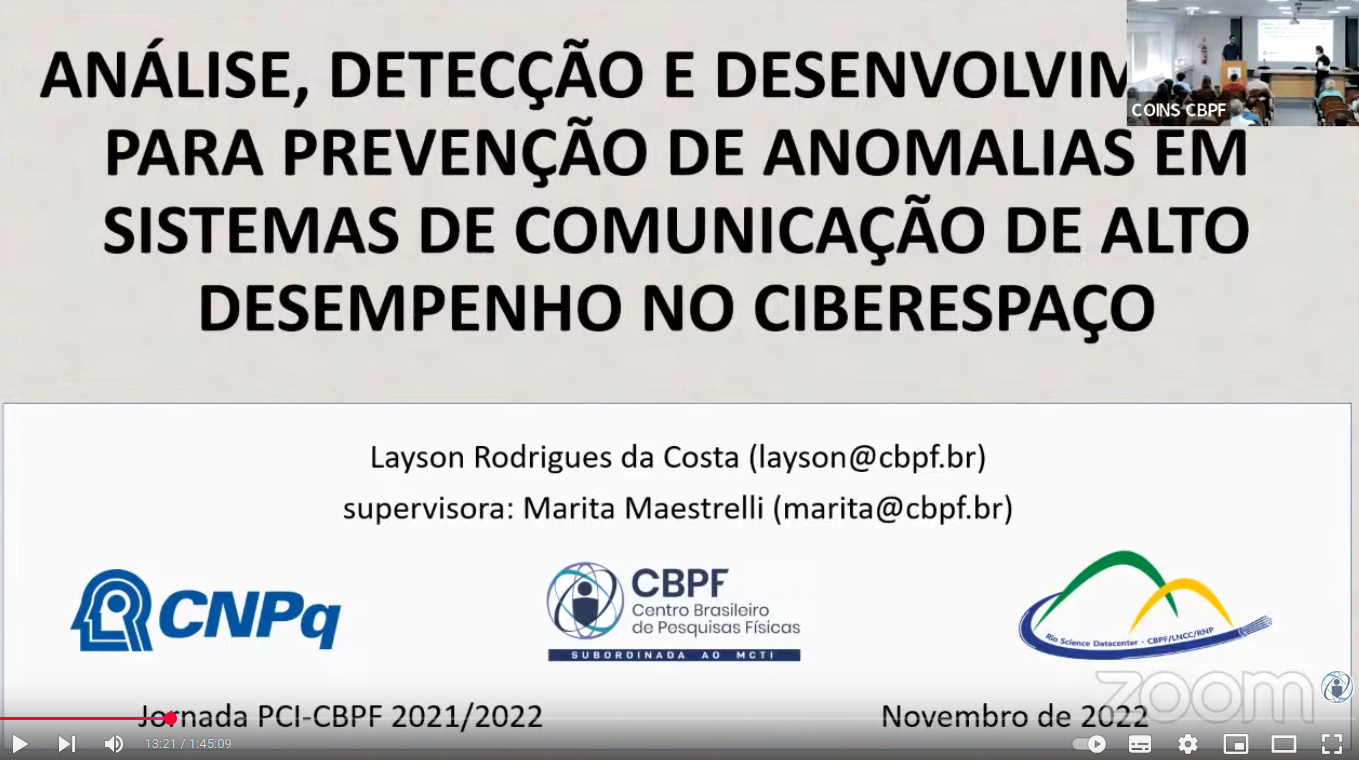
\includegraphics[width=0.75\linewidth]{Figuras/apresentacao-nfdump-nfsen-layson.png}
    \vspace{0.3cm}


\href{https://www.youtube.com/watch?v=vmK7_SBREm4}{\textcolor{blue}{Link: Apresentação no YouTube (Começa em 13:21)}}

\href{https://www.gov.br/cbpf/pt-br/pesquisa-e-desenvolvimento/capacitacao-institucional-pci/jornada/apresentacaolaysonrodrigues.pdf}{\textcolor{blue}{Link: Arquivo .pdf da apresentação}}

\end{frame}


